\documentclass[aspectratio=169]{beamer}
\setbeamertemplate{navigation symbols}{}
\usepackage{color,amsmath,comment, subfigure}
\usepackage{booktabs}
\usepackage{url}

%%%%%%%%%%%%%%%%%%%%%%%%%%
\title[]{Class 13: Respondent-driven sampling}
\author[]{Matthew J. Salganik}
\institute[]{Sociology 204: Social Networks\\Princeton University}
\date[]{
2/3 Estimation
\vfill
\begin{flushleft}
\vspace{0.6in}

\includegraphics[width=0.1\textwidth]{figures/cc.png}
\end{flushleft}

}

\begin{document}
%%%%%%%%%%%%%%%%%%%%%%%%%%%
\frame{\titlepage}
%%%%%%%%%%%%%%%%%%%%%%%%%%%
\begin{frame}

Respondent-driven sampling describes both:
\begin{itemize}
\item a method of data collection
\item a method of estimation
\end{itemize}

\end{frame}
%%%%%%%%%%%%%%%%%%%%%%%%%%%
\begin{frame}

To summarize years of work:\\
Under certain assumptions about the recruitment process, participants are selected with probability proportional to their degree.  For example, someone with 10 friends in the hidden population is twice as likely to be selected as someone with 5 friends.\\

\end{frame}
%%%%%%%%%%%%%%%%%%%%%%%%%%%
\frame{
\frametitle{Estimation: Assumptions}
4 key assumptions (but really 3)
\begin{itemize}
\item Population forms one connected component and ties are reciprocal
\item Sampling with replacement
\item People recruit randomly from their friends
\item Seed selected with probability proportion to their degree\\
\begin{itemize}
\item This assumption can be relaxed if the sample size is ``large''
\end{itemize}
\end{itemize}
}
%%%%%%%%%%%%%%%%%%%%%%%%%%
\frame{
\frametitle{Estimation: Consequences of assumptions}
\begin{figure}
\center
\includegraphics<1>[width=0.7\textwidth]{figures/rds_water_schematic_4nodes} %
\includegraphics<2>[width=0.7\textwidth]{figures/rds_water_schematic_4nodes_nodes} % 
\includegraphics<3>[width=0.7\textwidth]{figures/rds_water_schematic_4nodes_edges} %
\includegraphics<4>[width=0.7\textwidth]{figures/rds_water_schematic_4nodes_nodes} %
\end{figure}
}
%%%%%%%%%%%%%%%%%%%%%%%%%%%
\frame{
\frametitle{Seeds not drawn correctly}
\begin{figure}
\center
\includegraphics<1>[width=0.5\textwidth]{figures/rds_water_schematic_4nodes} %
\includegraphics<2>[width=0.5\textwidth]{figures/rds_water_schematic_4nodes_badseeds1} % 
\includegraphics<3>[width=0.5\textwidth]{figures/rds_water_schematic_4nodes_badseeds2} %
\includegraphics<4>[width=0.5\textwidth]{figures/rds_water_schematic_4nodes_badseeds3} %
\includegraphics<5>[width=0.5\textwidth]{figures/rds_water_schematic_4nodes_badseeds4} %
\includegraphics<6>[width=0.5\textwidth]{figures/rds_water_schematic_4nodes_badseeds5} %
\includegraphics<7>[width=0.5\textwidth]{figures/rds_water_schematic_4nodes_edges} %
\includegraphics<8>[width=0.5\textwidth]{figures/rds_water_schematic_4nodes_nodes} %
\end{figure}
}

\note{
be sure to say after many steps . . . . 
}
%%%%%%%%%%%%%%%%
\begin{frame}

If people are selected with probability proportional to degree (and we can measure their degree), then we can weight people by the inverse of their degree.

$$\hat{\bar{y}} = \frac{ \sum_{i=1}^{n} y_i / d_i }{ \sum_{i=1}^{n} 1/ d_i}$$
where
\begin{itemize}
\item $\hat{\bar{y}}$: estimated average infection rate
\item $y_i$: infection status of person $i$
\item $d_i$: degree of person $i$
\end{itemize}

\end{frame}
%%%%%%%%%%%%%%%%%%%%%%%%%%
\begin{frame}

$$\hat{\bar{y}} = \frac{ \sum_{i=1}^{n} y_i / d_i }{ \sum_{i=1}^{n} 1/ d_i}$$

\begin{tabular}{rr}
Infected ($y_i$) & Degree ($d_i$)\\
0 & 10\\
1 & 20\\
1 & 35\\
0 & 5\\
0 & 10\\
1 & 30\\
0 & 5\\
1 & 40\\
0 & 10\\
1 & 20\\
\end{tabular}
\pause
\begin{itemize}
\item sample mean = 0.5 \pause
\item $\hat{\bar{y}} = \frac{ 0 + 1/ 20 + 1/35 + 0 + 0 + 1/30 + 0 + 1/40 + 0 + 1/20 }{ 1/10 + 1/20 + 1/35 + 1/5 + 1/10 + 1/30 + 1/5 + 1/40 + 1/10 + 1/20 } \approx 0.19 / 0.89 \approx  0.21$
\end{itemize}

\note{Sometimes degree can be related to length of time in the hidden population, which can be related to risk and therefore probability of infection}

\end{frame}
%%%%%%%%%%%%%%%%%%%%%%%%%%%%%%%%%%%%
\frame{
\frametitle{But . . . }

To summarize years of work:\\
The structure of real social networks may be unfavorable to RDS.  In particular, it may lead to estimates with high sample-to-sample variability, which makes the estimates less useful.

}
%%%%%%%%%%%%%%%%%%%%%%%%%%%
\frame{
\frametitle{RDS as MCMC Importance Sampling}

Goel and Salganik (2009) introduced a connection between respondent-driven sampling and Markov Chain Monte Carlo importance sampling.  By making this connection we can establish two things:

\vfill
\begin{itemize}
\item Community structure (e.g., cohesive subgroups) in the social network increases the variance of RDS estimates. In particular,``bottlenecks'' anywhere in the network may degrade estimates---bottlenecks need not be directly related to the characteristics being studied.
\item A design that incorporates multiple recruitment increases the variance of RDS estimates.
\end{itemize}
}
%%%%%%%%%%%%%%%%%%%%%%%%%%%%
\section{Toy example}
\frame{
\frametitle{An Example: Bottlenecks}

Consider a population consisting of two equal-sized groups where \textit{within-group} edges are more likely than \textit{between-group} edges.  For example, street-based and agency-based sex workers in Belgrade (Simic, et al 2007).
\begin{center}
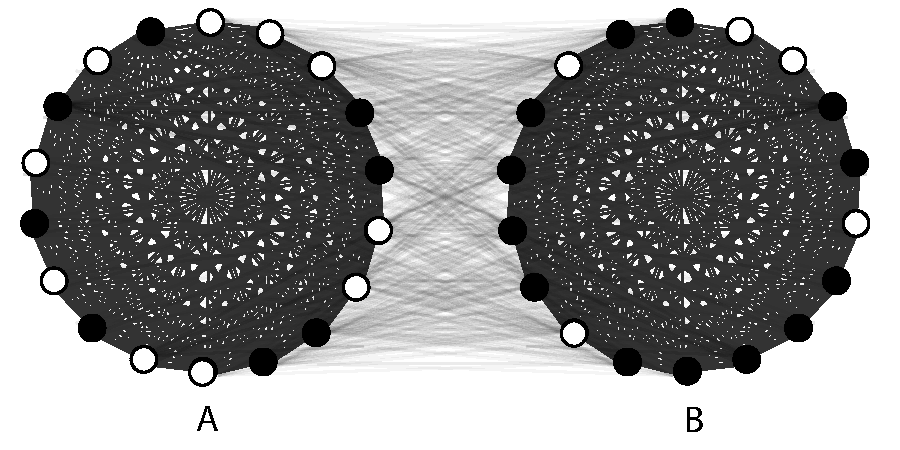
\includegraphics[width=0.5\textwidth]{figures/network}\\
White nodes are infected; black nodes are healthy.
\end{center}
Focusing solely on the connection between healthy and infected overlooks the key structural feature of this network.  \textcolor{blue}{Bottlenecks need not be directly related to the characteristic being studied}.
}
%%%%%%%%%%%%%%%%%%%%%%%%%%%%
\frame{
\frametitle{An Example: Bottlenecks}

\setcounter{subfigure}{0}
\begin{figure}
  \centering
     \subfigure[]{
     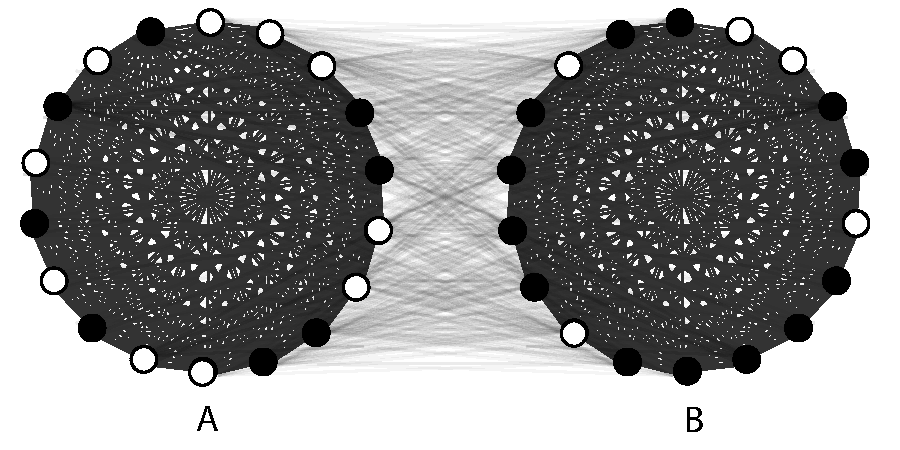
\includegraphics[width=0.45\textwidth]{figures/network}}
  \hspace{0in}
    \subfigure[]{
    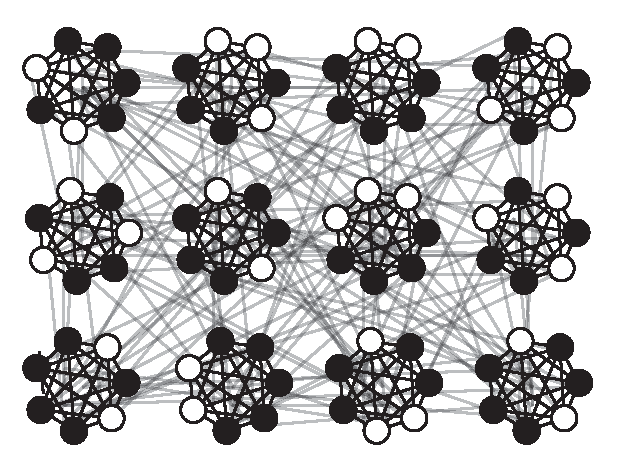
\includegraphics[width=0.45\textwidth]{figures/network3}}
\end{figure}
More subtle bottlenecks can cause the same problem.  These two networks are the same in terms of RDS variance. 
}
%%%%%%%%%%%%%%%%
\frame{
\frametitle{An Example: Multiple recruitment}
Multiple recruitment is needed for the sampling process to continue in practice, but it increases the variance of the estimates by increasing the dependence between sample observations.
\begin{center}
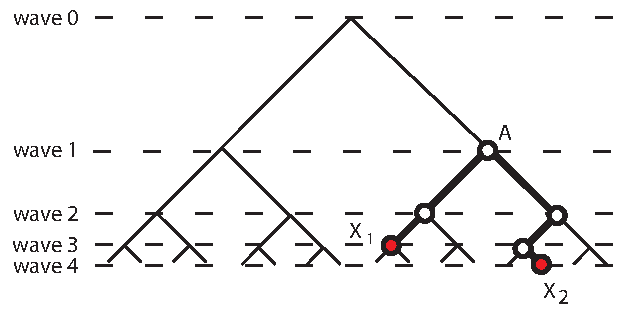
\includegraphics[width=0.5\textwidth]{figures/recruitment_net}
\end{center}
The effective sample size is smaller than the observed sample size.   In other words, you have less information than you think.
}
%%%%%%%%%%%%%%%%%%%%%%%%%%%%
\frame{
\frametitle{Toy example}

To summarize our findings for this hypothetical population, we compare three sampling situations: \textcolor{red}{simple random sampling}, \textcolor{blue}{RDS with single recruitment}, and \textcolor{green}{RDS with multiple recruitment}. We use parameters $p_A = .1$, $p_B = .3$, $c = .1$, sample size $n = 500$, and 2 seeds chosen independently from the stationary distribution (more general results in our paper). Multiple recruitment is based on a branching process with offspring distribution:
\begin{center}
\begin{tabular}{lcccc}
\toprule
& \multicolumn{4}{c}{Number of recruits}\\
\cmidrule{2-5}
 & 0 & 1 & 2 & 3 \\ 
\midrule
Probability & 1/3 & 1/6 & 1/6 & 1/3\\
\bottomrule
\end{tabular}
\end{center}
This recruitment distribution is based on RDS data from the Frost, et. al. (2006) study of drug-injectors in Tijuana and Ciudad Juarez.
}
%%%%%%%%%%%%%%%%%%%%%%%%%%%%%%
\frame{
\small
\begin{center}
\includegraphics<1>[width=0.6\textwidth]{figures/example_hist_1}
\includegraphics<2>[width=0.6\textwidth]{figures/example_hist_2}
\includegraphics<3>[width=0.6\textwidth]{figures/example_hist_3}
\end{center}
\vfill
\begin{center}
\begin{tabular}{lc}
& effective sample size \\ \hline
\textcolor{red}{Simple Random Sampling} & 500 \\
\onslide<2->{\textcolor{blue}{RDS -- Single Recruitment} & 335\\}
\onslide<3->{\textcolor{green}{RDS -- Multiple Recruitment} & 136\\}
\end{tabular}
\end{center}
}
%%%%%%%%%%%%%%%%%%%%%%%%%%%%%%
\begin{frame}

\begin{center}
\includegraphics<1>[width=0.7\textwidth]{figures/goel_respondent_2009_title}
\end{center}

\vfill
\url{https://doi.org/10.1002/sim.3613}
\end{frame}
%%%%%%%%%%%%%%%%%%%%%%%%%%%%%%
\frame{
\frametitle{What about real networks?}
Hopefully the toy example helps to build intuition. But what about in real networks?  We quickly run into a data problem:
\begin{itemize}
\item Complete social network data for large networks
\item Demographic information for each node
\end{itemize}
\pause
\vfill
We have found 2 such sources:
\begin{itemize}
\item Add Health
\item Project 90
\end{itemize}
}
%%%%%%%%%%%%%%%%%%%%%%%%%%%%%%
\frame{
\frametitle{A note on these simulations}

The following simulations will assume that all RDS assumptions are met.  This represents a useful case to examine, but of course, many assumptions will not be met in practice.
\begin{itemize}
\item sample size of 500
\item 10 seeds chosen with probability proportional to degree (i.e., from stationary distribution)
\item Offspring distribution based on Frost et al. (2006):
\begin{center}
\begin{tabular}{lcccc}
\toprule
& \multicolumn{4}{c}{Number of recruits}\\
\cmidrule{2-5}
 & 0 & 1 & 2 & 3 \\ 
\midrule
Probability & 1/3 & 1/6 & 1/6 & 1/3\\
\bottomrule
\end{tabular}
\end{center}
\end{itemize}
}
%%%%%%%%%%%%%%%%%%%%%%%%%%%%%%%
\frame{
\frametitle{Add Health}
National Longitudinal Study of Adolescent Health (Add Health), Source: UNC-Pop. Center
\begin{itemize}
\item 84 schools with giant components ranging from 25 to 2,539 (mean=860).
\item Respondents were asked to chose from a roster \textcolor{blue}{up to 5 male friends and up to 5 female friends}.  All responses were symmetrized and degrees range from 1 to 38 (mean=7).
\begin{center}
\includegraphics<1>[width=0.4\textwidth]{figures/addhealth_degree_dist}
\end{center}
\end{itemize}
}
%%%%%%%%%%%%%%%%%%%%%%%%%%%%
\frame{
\frametitle{Add Health: Estimates, prop. non-white}
\begin{center}
\includegraphics<1>[width=0.55\textwidth]{figures/addhealth_nonwhite_N_allschools_true_slides}
\includegraphics<2>[width=0.55\textwidth]{figures/addhealth_nonwhite_N_allschools_estimates_slides}
\includegraphics<3>[width=0.55\textwidth]{figures/addhealth_nonwhite_N_allschools_estimates_var_slides}
\end{center}
}
%%%%%%%%%%%%%%%%%%%%%%%%%%%%%%
\frame{
\frametitle{Add Health: Estimates, prop. female}
\begin{center}
\includegraphics<1>[width=0.55\textwidth]{figures/addhealth_female_N_allschools_true_slides}
\includegraphics<2>[width=0.55\textwidth]{figures/addhealth_female_N_allschools_estimates_slides}
\includegraphics<3>[width=0.55\textwidth]{figures/addhealth_female_N_allschools_estimates_var_slides}
\end{center}
}
%%%%%%%%%%%%%%%%%%%%%%%%%%%%%
\frame{
\frametitle{Design effect}
Quantify variability with design effect:
$deff = \frac{var(\hat{p}_{RDS})}{var(\hat{p}_{SRS})}$

\begin{itemize}
\item Can be thought of as a measure of the \textcolor{blue}{``relative efficiency''} of the sampling methods.  Values bigger than 1 mean that RDS is less efficient than simple random sampling. \pause
\item Note that design effect is a property the estimator for a trait in a population, not just a population.  For example, the design effect for prop. female may be different from design effect for prop. non-white.
\end{itemize}

}
%%%%%%%%%%%%%%%%%%%%%%%%%%%%
\frame{
\frametitle{Add Health: Design effects}
\begin{figure}
  \centering
  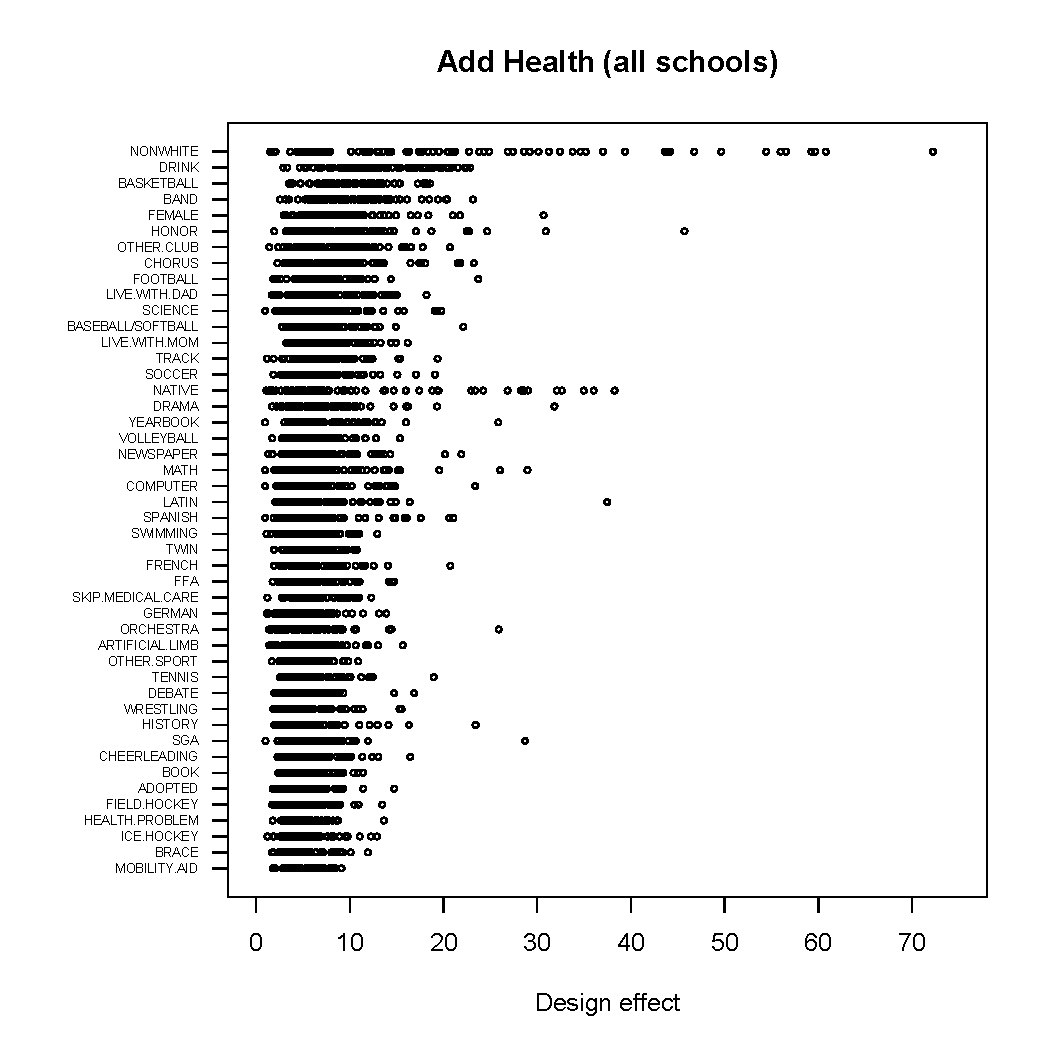
\includegraphics[height=0.7\textheight]{figures/addhealth_de_alltraits_allschools_strip}
\end{figure}
\textcolor{blue}{The median design effect is about 5} and socially salient characteristics are even higher.
}
%%%%%%%%%%%%%%%%%%%%%%%%%%%
\begin{frame}
\frametitle{Add Health: Design effects}
Design effect of 5 means: 
\begin{itemize}
\item RDS sample of 500 have same variance as a simple random sample of size 100.
\item RDS confidence intervals should be about 2 times ($\sqrt{5}$) wider.
\item It will be very difficult to reliably detect change over time (from 40\% to 30\% requires $n=1750$)
\end{itemize}

\end{frame}
%%%%%%%%%%%%%%
\frame{
\frametitle{Limitations of Add Health data}
\begin{itemize}
\item Some schools were very small. 
\pause
\item Fixed choice design limited out-degree. 
\pause
\item Networks of high school students might be different from networks of drug injectors, sex workers, or other hidden populations.
\end{itemize}
}
%%%%%%%%%%%%%%%%%%%%%%%%%%%%%%%
\frame{
\frametitle{An Overview of Project 90}
Project 90 was a multi-year study that mapped the connections between sex workers, drug injectors, and their sexual partners, beginning in Colorado Springs from 1988-1992.\pause
\begin{itemize}
\item The entire Project 90 network contains 5,492 individuals and 21,644 edges, representing \textcolor{blue}{social, sexual, and/or drug affiliation}. 
\pause
\item We restrict attention to the giant component of this network, consisting of \textcolor{blue}{4,430 nodes and 18,407 edges}. 
\pause
\item The median degree of an individual in the giant component is 6, with a degree range of 1 to 159. 
\end{itemize}
\vfill
We thank the Project 90 Team, especially Steve Muth and John Potterat, for sharing the data.
}
%%%%%%%%%%%%%%%%%%%%%%%%%%%%%%%
\frame{
\frametitle{Project 90, prop. female}
\begin{center}
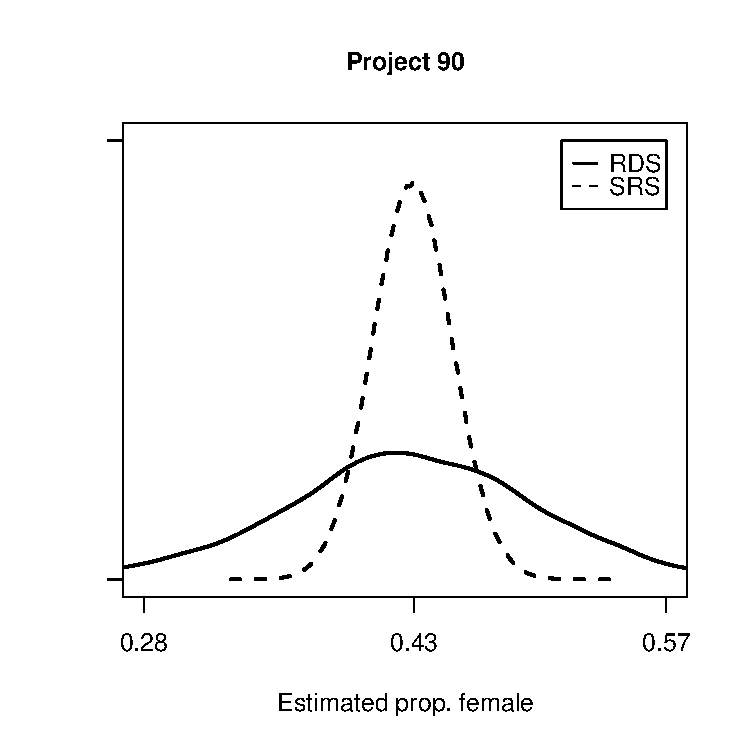
\includegraphics[width=0.5\textwidth]{figures/proj90_dist_prop_female}
\end{center}
Estimating of prop. female are unbiased, but the design effect is about 11.
}
%%%%%%%%%%%%%%%%%%%%%%%%%%%%%%%
\frame{
\frametitle{Project 90, prop. non-white}
\begin{center}
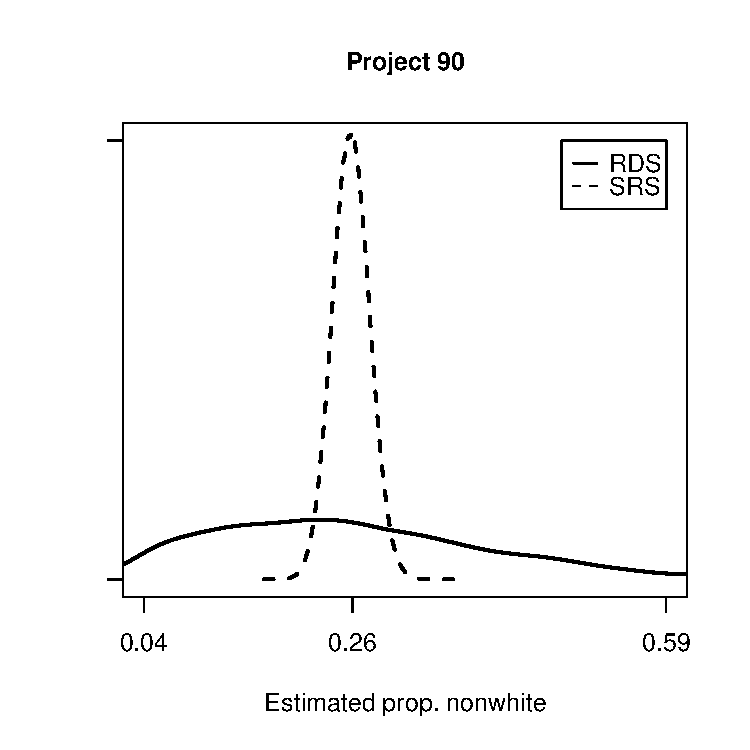
\includegraphics[width=0.5\textwidth]{figures/proj90_dist_prop_nonwhite}
\end{center}
Estimates of prop. non-white are unbiased, but the design effect is about 57.
}
%%%%%%%%%%%%%%%%%%%%%%%%%%%%%%%
\frame{
\frametitle{Project 90, Why are the estimates so variable?}

\textcolor{blue}{There is considerable community structure in this dataset}: The giant component partitions into two groups of sizes 1,076 and 3,354 individuals, with few between-group edges (the conductance is 0.13), and such that the percentage of non-Whites in the former group is 55.6\% and in the latter 12.2\%.
}
%%%%%%%%%%%%%%%%%%%%%%%%%%%%%%
\frame{
\frametitle{Project 90, Why are the estimates so variable?}

Even worse, the source of this community structure is not clear (to us), so it may be hard to detect just with sample information.\\

Analogous to our toy example, it is not segregation directly between Whites and non-Whites, for example, that leads to poor RDS estimates. To the contrary, \textcolor{blue}{Whites and non-Whites, and men and women, on the whole are well-connected in this network}.
%In terms of conductance, the male/female division yields a value of 0.49, and the White/non-White division a value of 0.32.
\vfill
This is what you could see in a sample:\\
\begin{center}
\begin{tabular}{lcc}
\toprule
 & White & Non-White\\
\cmidrule{2-3} 
White & 282 & 63\\
Non-White & 77 & 68\\
\bottomrule
\end{tabular}
\end{center}
}
%%%%%%%%%%%%%%%%%%%%%%%%%%%%%%%
\frame{
\frametitle{Problems with Project 90}
\begin{itemize}
\item Missing edges
\item Missing nodes
\item Many nodes with degree 1 (i.e., very ``leafy'')
\end{itemize}
\begin{center}
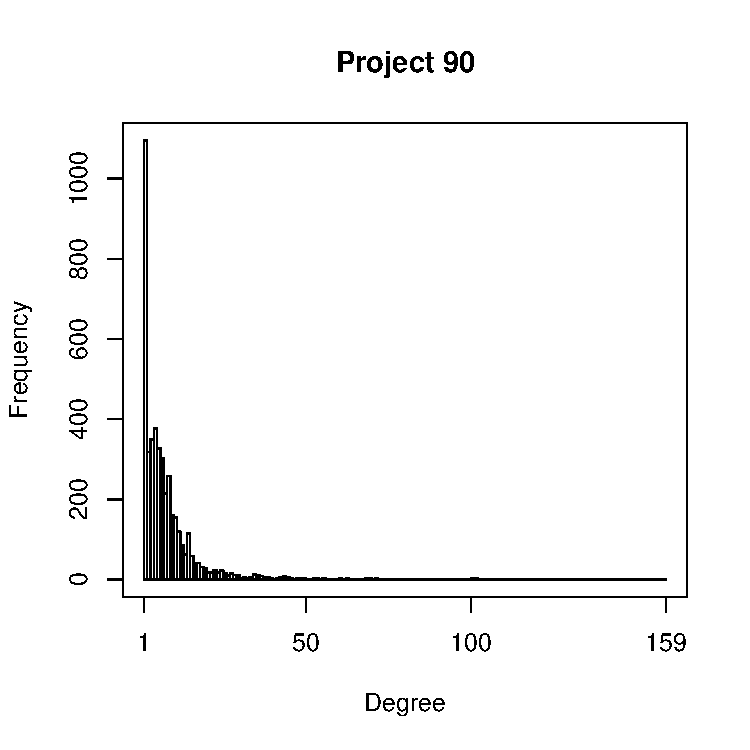
\includegraphics[width=0.4\textwidth]{figures/proj90_degree_dist}
\end{center}
}
%%%%%%%%%%%%%%%%%%%%%%%%%%%%%
\begin{frame}

But what about. . . . . ?\\
We can address these questions with robustness checks.

\end{frame}
%%%%%%%%%%%%%%%%%%%%%%%%%%%
\frame{
\frametitle{Robustness checks: RDS I and RDS II}
\begin{figure}
  \centering
  \includegraphics<1>[height=0.65\textheight]{figures/figure_s1}
\end{figure}
$\rightarrow$ Similar results for RDS I and RDS II estimators.
}
%%%%%%%%%%%%%%%%%%%%%%%%%%%%%%%
\frame{
\frametitle{Robustness checks: Leaves in Project 90}
\begin{figure}
  \centering
  \includegraphics<1>[width=0.9\textwidth]{figures/figure_s2}
\end{figure}
$\rightarrow$ Similar results with and without leaves.
}
%%%%%%%%%%%%%%%%%%%%%%%%%%%%%%%
\frame{
\frametitle{Robustness check: High schools \& joint middle/high schools}
\begin{figure}
  \centering
  \includegraphics<1>[height=0.65\textheight]{figures/figure_s3}
\end{figure}
$\rightarrow$ Similar results in high schools and joint middle and high schools.
}
%%%%%%%%%%%%%%%%%%%%%%%%%%%%%%%
\frame{
\frametitle{Robustness check: Reciprocity in constructing network}
\begin{figure}
  \centering
  \includegraphics<1>[height=0.65\textheight]{figures/figure_s4}
\end{figure}
$\rightarrow$ Median design effect increases to about 19 when using fully reciprocal network.
}
%%%%%%%%%%%%%%%%%%%%%%%%%%%%%%%
\frame{
\frametitle{Robustness check: Not just small schools or rare traits}
\begin{figure}
  \centering
  \includegraphics<1>[width=0.9\textwidth]{figures/figure_s5}
\end{figure}
$\rightarrow$ High design effects are not just in small schools or for rare traits.
}
%%%%%%%%%%%%%%%%%%%%%%%%%%%%%%
\begin{frame}
\frametitle{Robustness checks}

Based on:
\begin{itemize}
\item Two distinct sources of data
\item More than 3,000 network/trait combinations (84 schools $\times$ 46 traits + 1 Project 90 $\times$ 13 traits) % 3,877
\item Several robustness checks
\end{itemize}

it seems that:
\begin{itemize}
\item RDS estimates are much less precise than previously believed and this result seems pretty robust. \pause
\item Estimates are so imprecise that \textcolor{blue}{it seems difficult to reliably detect change over time}.  For example, if we assume a design effect of 5, to reliably detect a drop in risk behavior from 40\% prevalence to 30\% prevalence ($\alpha=0.05, \beta=0.8)$ would require samples of about 1750 at both time points. \pauses
\end{itemize}

\end{frame}
%%%%%%%%%%%%%%%%%
\begin{frame}
\frametitle{More details}

\begin{center}
  
\includegraphics[width=0.9\textwidth]{figures/goel_assessing_2010_title}
\end{center}

\vfill
\url{https://doi.org/10.1073/pnas.1000261107}

\end{frame}
%%%%%%%%%%%%%%%%%%
\begin{frame}

How can we improve respondent-driven sampling?

\end{frame}
%%%%%%%%%%%%%%%%%%%%%%%%%%%%%%

\end{document}
